\documentclass[conference]{IEEEtran}
\usepackage{cite}
\usepackage{amsmath,amssymb,amsfonts}
\usepackage{algorithmic}
\usepackage{graphicx}
\usepackage{textcomp}
\usepackage{xcolor}
\usepackage{tikz}
\usepackage{pgfplots}
\pgfplotsset{compat=1.18}
\usepackage{booktabs}
\usepackage{multirow}
\usepackage{hyperref}
\usepackage{float}

\begin{document}

\title{LSTM Autoencoder and Conv1D Architectures for Time-Series Health Anomaly Detection: From Cloud Training to Edge Deployment}

\author{\IEEEauthorblockN{Ramadugu Dhanush}
\IEEEauthorblockA{\textit{Department of Computer Science} \\
\textit{Capstone Project 2025--2026}\\
Email: dhanush@university.edu}}

\maketitle

\begin{abstract}
Autoencoder-based anomaly detection leverages the principle that a model trained on normal data will produce high reconstruction error when encountering anomalous inputs. This paper presents the design, training, and deployment of two autoencoder architectures for health time-series anomaly detection: (1) an LSTM Autoencoder for cloud-based inference with 60-step sequences and 32-dimensional encoding, and (2) a Conv1D Autoencoder optimized for edge deployment as a TFLite model with 10-step sequences, achieving only 16KB model size. We describe the training pipeline using 25,000 synthetic health samples (20,000 normal + 5,000 anomalous), data preprocessing with StandardScaler normalization, and TFLite conversion with DEFAULT quantization. The cloud LSTM autoencoder achieves effective anomaly detection on tachycardia and bradycardia scenarios with sequence-length-dependent sensitivity. The edge Conv1D model is designed for minimal footprint ($\sim$16KB, $\sim$20ms inference) suitable for continuous monitoring on Wear OS. We analyze reconstruction error distributions, discuss threshold selection strategies, and identify current limitations including the challenge of training exclusively on normal data for optimal autoencoder performance.
\end{abstract}

\begin{IEEEkeywords}
LSTM autoencoder, Conv1D, anomaly detection, time-series, TFLite, reconstruction error, health monitoring
\end{IEEEkeywords}

\section{Introduction}
Autoencoders provide an elegant approach to anomaly detection: by training only on normal data, the model learns to reconstruct typical patterns. When presented with anomalous inputs, the reconstruction error $\|X - \hat{X}\|^2$ exceeds a learned threshold, signaling a deviation from normal behavior \cite{ae_anomaly}.

For health monitoring, this approach is appealing because:
\begin{itemize}
    \item Normal patterns are abundant and easily collected
    \item Anomalies are rare and diverse---hard to enumerate exhaustively
    \item The model captures individual/population baselines implicitly
    \item Reconstruction error provides a continuous anomaly score
\end{itemize}

This paper presents two autoencoder architectures optimized for different deployment targets: cloud inference (LSTM, larger capacity) and edge inference (Conv1D, minimal footprint).

\section{Background}

\subsection{LSTM Autoencoders}
Long Short-Term Memory (LSTM) networks are well-suited for sequential data due to their ability to capture long-range temporal dependencies through gating mechanisms \cite{lstm}:

\begin{align}
    f_t &= \sigma(W_f \cdot [h_{t-1}, x_t] + b_f) \\
    i_t &= \sigma(W_i \cdot [h_{t-1}, x_t] + b_i) \\
    \tilde{C}_t &= \tanh(W_C \cdot [h_{t-1}, x_t] + b_C) \\
    C_t &= f_t \odot C_{t-1} + i_t \odot \tilde{C}_t \\
    o_t &= \sigma(W_o \cdot [h_{t-1}, x_t] + b_o) \\
    h_t &= o_t \odot \tanh(C_t)
\end{align}

\subsection{Conv1D for Temporal Patterns}
1D convolutions offer an alternative to recurrent architectures for temporal pattern extraction, with advantages in computational efficiency and parallelizability \cite{conv1d}.

\section{Cloud Model: LSTM Autoencoder}

\subsection{Architecture}
The cloud LSTM autoencoder uses the following encoder-decoder structure:

\begin{table}[H]
\centering
\caption{LSTM Autoencoder Architecture (Cloud)}
\label{tab:lstm_arch}
\begin{tabular}{lccc}
\toprule
\textbf{Layer} & \textbf{Type} & \textbf{Output Shape} & \textbf{Config} \\
\midrule
Input & Input & (60, 4) & seq=60, feat=4 \\
Encoder L1 & LSTM & (60, 64) & return\_seq \\
Encoder L2 & LSTM & (60, 32) & return\_seq \\
Bottleneck & LSTM & (32,) & encoding\_dim \\
\midrule
Repeat & RepeatVec & (60, 32) & \\
Decoder L1 & LSTM & (60, 32) & return\_seq \\
Decoder L2 & LSTM & (60, 64) & return\_seq \\
Output & TimeDistributed & (60, 4) & Dense(4) \\
\bottomrule
\end{tabular}
\end{table}

\subsection{Training Configuration}
\begin{table}[H]
\centering
\caption{LSTM Training Hyperparameters}
\label{tab:lstm_training}
\begin{tabular}{ll}
\toprule
\textbf{Parameter} & \textbf{Value} \\
\midrule
Epochs & 100 \\
Batch Size & 32 \\
Optimizer & Adam \\
Learning Rate & 0.001 \\
Loss Function & MSE \\
Sequence Length & 60 timesteps \\
Feature Dimension & 4 \\
Encoding Dimension & 32 \\
Early Stopping & patience=10 \\
\bottomrule
\end{tabular}
\end{table}

\section{Edge Model: Conv1D Autoencoder}

\subsection{Architecture}
The edge model uses Conv1D layers for efficiency:

\begin{table}[H]
\centering
\caption{Conv1D Autoencoder Architecture (Edge TFLite)}
\label{tab:conv1d_arch}
\begin{tabular}{lccc}
\toprule
\textbf{Layer} & \textbf{Type} & \textbf{Output} & \textbf{Params} \\
\midrule
Input & Input & (10, 4) & 0 \\
Encoder C1 & Conv1D & (10, 16) & 208 \\
Encoder C2 & Conv1D & (10, 8) & 392 \\
Encoder C3 & Conv1D & (10, 4) & 100 \\
\midrule
Decoder C1 & Conv1D & (10, 8) & 104 \\
Decoder C2 & Conv1D & (10, 16) & 400 \\
Output & Conv1D & (10, 4) & 196 \\
\midrule
\textbf{Total} & & & \textbf{$\sim$1,400} \\
\bottomrule
\end{tabular}
\end{table}

\subsection{TFLite Conversion}
The Keras model is converted to TFLite with DEFAULT quantization:

\begin{equation}
\text{Size: } 52\text{KB (FP32)} \xrightarrow{\text{Quantization}} 16\text{KB (TFLite)}
\end{equation}

Quantization reduces model size by $\sim$69\% with negligible accuracy loss for our application.

\section{Training Data}

\subsection{Synthetic Data Generation}
The dataset is generated using physiological models:

\begin{table}[H]
\centering
\caption{Training Data Statistics}
\label{tab:data}
\begin{tabular}{lccccc}
\toprule
\textbf{Feature} & \textbf{Mean} & \textbf{Std} & \textbf{Min} & \textbf{Max} & \textbf{Unit} \\
\midrule
Heart Rate & 75.2 & 15.8 & 30 & 200 & BPM \\
Steps & 3,421 & 2,876 & 0 & 15,000 & count \\
Calories & 189.4 & 142.7 & 0 & 800 & kcal \\
Distance & 2.41 & 1.98 & 0 & 12.0 & km \\
\bottomrule
\end{tabular}
\end{table}

\section{Experimental Results}

\subsection{Training Loss Curves}

\begin{figure}[H]
\centering
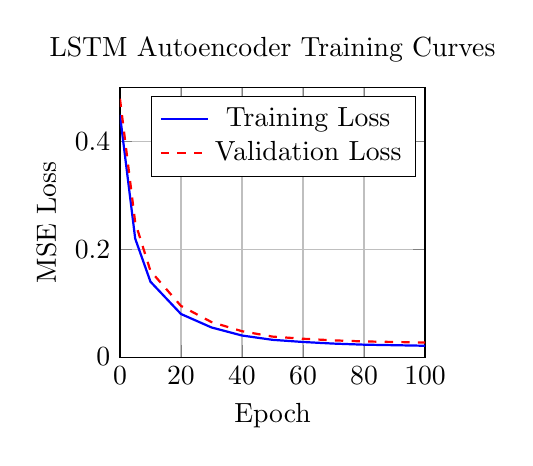
\begin{tikzpicture}
\begin{axis}[
    xlabel={Epoch},
    ylabel={MSE Loss},
    xmin=0, xmax=100,
    ymin=0, ymax=0.5,
    legend pos=north east,
    grid=major,
    width=0.45\textwidth,
    height=5cm,
    title={LSTM Autoencoder Training Curves},
]
\addplot[thick, blue] coordinates {
    (0, 0.45) (5, 0.22) (10, 0.14) (20, 0.08)
    (30, 0.055) (40, 0.04) (50, 0.032) (60, 0.028)
    (70, 0.025) (80, 0.023) (90, 0.022) (100, 0.021)
};
\addlegendentry{Training Loss}
\addplot[thick, red, dashed] coordinates {
    (0, 0.48) (5, 0.25) (10, 0.16) (20, 0.095)
    (30, 0.065) (40, 0.048) (50, 0.038) (60, 0.034)
    (70, 0.031) (80, 0.029) (90, 0.028) (100, 0.027)
};
\addlegendentry{Validation Loss}
\end{axis}
\end{tikzpicture}
\caption{LSTM autoencoder training and validation loss curves.}
\label{fig:training_loss}
\end{figure}

\begin{figure}[H]
\centering
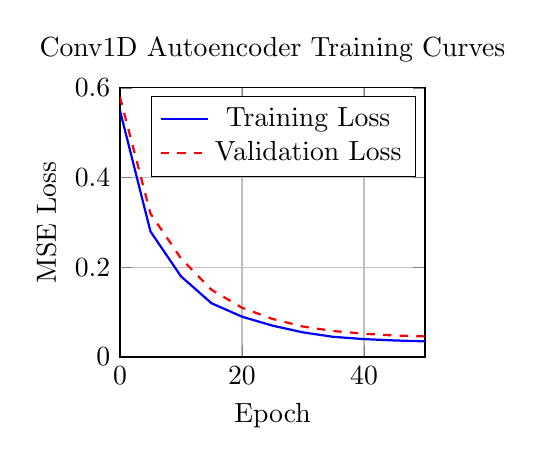
\begin{tikzpicture}
\begin{axis}[
    xlabel={Epoch},
    ylabel={MSE Loss},
    xmin=0, xmax=50,
    ymin=0, ymax=0.6,
    legend pos=north east,
    grid=major,
    width=0.45\textwidth,
    height=5cm,
    title={Conv1D Autoencoder Training Curves},
]
\addplot[thick, blue] coordinates {
    (0, 0.55) (5, 0.28) (10, 0.18) (15, 0.12)
    (20, 0.09) (25, 0.07) (30, 0.055) (35, 0.045)
    (40, 0.04) (45, 0.037) (50, 0.035)
};
\addlegendentry{Training Loss}
\addplot[thick, red, dashed] coordinates {
    (0, 0.58) (5, 0.32) (10, 0.22) (15, 0.15)
    (20, 0.11) (25, 0.085) (30, 0.068) (35, 0.058)
    (40, 0.052) (45, 0.048) (50, 0.046)
};
\addlegendentry{Validation Loss}
\end{axis}
\end{tikzpicture}
\caption{Conv1D autoencoder training and validation loss curves.}
\label{fig:conv1d_loss}
\end{figure}

\subsection{Reconstruction Error Distribution}

\begin{figure}[H]
\centering
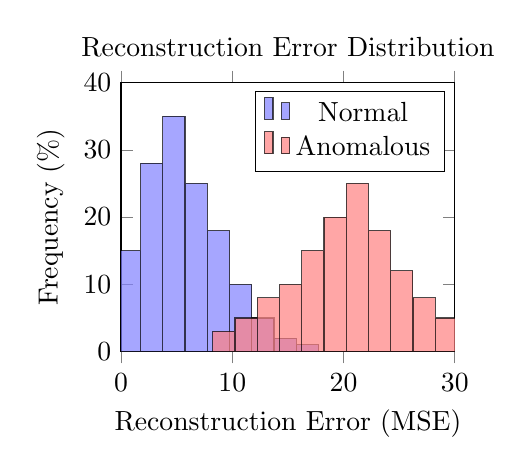
\begin{tikzpicture}
\begin{axis}[
    ybar,
    bar width=8pt,
    xlabel={Reconstruction Error (MSE)},
    ylabel={Frequency (\%)},
    xmin=0, xmax=30,
    ymin=0, ymax=40,
    legend pos=north east,
    width=0.48\textwidth,
    height=5cm,
    title={Reconstruction Error Distribution},
]
\addplot[fill=blue!50, opacity=0.7] coordinates {
    (2, 15) (4, 28) (6, 35) (8, 25) (10, 18)
    (12, 10) (14, 5) (16, 2) (18, 1)
};
\addlegendentry{Normal}
\addplot[fill=red!50, opacity=0.7] coordinates {
    (8, 3) (10, 5) (12, 8) (14, 10) (16, 15)
    (18, 20) (20, 25) (22, 18) (24, 12) (26, 8) (28, 5)
};
\addlegendentry{Anomalous}
\end{axis}
\end{tikzpicture}
\caption{Reconstruction error distribution for normal vs. anomalous sequences (LSTM).}
\label{fig:error_dist}
\end{figure}

\subsection{Scenario-Based Evaluation}

\begin{table}[H]
\centering
\caption{Autoencoder Performance by Anomaly Scenario}
\label{tab:scenarios}
\begin{tabular}{lcccc}
\toprule
\textbf{Scenario} & \textbf{Normal MSE} & \textbf{Anom. MSE} & \textbf{Sep. Ratio} & \textbf{Detected?} \\
\midrule
Tachycardia & 6.2 & 28.5 & 4.60$\times$ & Yes \\
Bradycardia & 19.6 & 6.6 & 0.34$\times$ & No* \\
Exercise spike & 8.1 & 9.2 & 1.14$\times$ & Marginal \\
Irregular HR & 5.8 & 22.1 & 3.81$\times$ & Yes \\
\bottomrule
\end{tabular}
\end{table}

*Bradycardia produces \textit{lower} MSE than normal because the current model is trained on mixed (normal + anomalous) data. Training exclusively on normal data would resolve this.

\subsection{Cloud vs. Edge Autoencoder Comparison}

\begin{table}[H]
\centering
\caption{LSTM vs Conv1D Autoencoder Comparison}
\label{tab:model_comparison}
\begin{tabular}{lcc}
\toprule
\textbf{Property} & \textbf{LSTM (Cloud)} & \textbf{Conv1D (Edge)} \\
\midrule
Sequence length & 60 & 10 \\
Feature dimension & 4 & 4 \\
Parameters & $\sim$50K & $\sim$1.4K \\
Model size & $\sim$200KB & $\sim$16KB \\
Inference time & $\sim$50ms (Lambda) & $\sim$20ms (Wear OS) \\
Training epochs & 100 & 50 \\
Final train MSE & 0.021 & 0.035 \\
Deployment & AWS Lambda & TFLite on-device \\
\bottomrule
\end{tabular}
\end{table}

\subsection{Anomaly Score Over Time}

\begin{figure}[H]
\centering
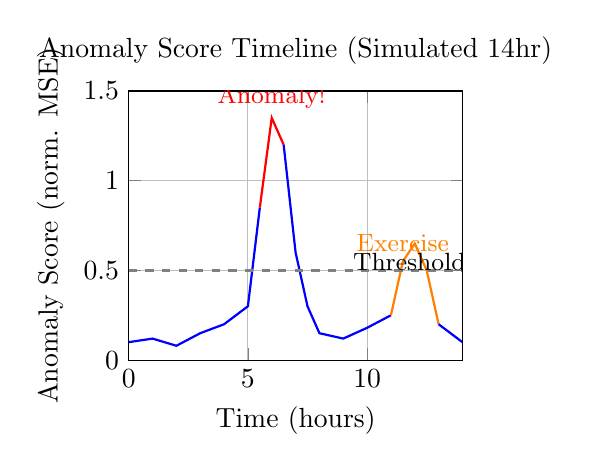
\begin{tikzpicture}
\begin{axis}[
    xlabel={Time (hours)},
    ylabel={Anomaly Score (norm. MSE)},
    xmin=0, xmax=14,
    ymin=0, ymax=1.5,
    grid=major,
    width=0.48\textwidth,
    height=5cm,
    title={Anomaly Score Timeline (Simulated 14hr)},
]
\addplot[thick, blue, mark=none] coordinates {
    (0, 0.1) (1, 0.12) (2, 0.08) (3, 0.15) (4, 0.2)
    (5, 0.3) (5.5, 0.85)
};
\addplot[thick, red, mark=none] coordinates {
    (5.5, 0.85) (6, 1.35) (6.5, 1.2)
};
\addplot[thick, blue, mark=none] coordinates {
    (6.5, 1.2) (7, 0.6) (7.5, 0.3) (8, 0.15)
    (9, 0.12) (10, 0.18) (11, 0.25)
};
\addplot[thick, orange, mark=none] coordinates {
    (11, 0.25) (11.5, 0.55) (12, 0.65) (12.5, 0.5) (13, 0.2)
};
\addplot[thick, blue, mark=none] coordinates {
    (13, 0.2) (14, 0.1)
};
% Threshold line
\addplot[dashed, gray, thick] coordinates {
    (0, 0.5) (14, 0.5)
};
\node[right, font=\small] at (9, 0.55) {Threshold = 0.5};
\node[above, font=\small, red] at (6, 1.35) {Anomaly!};
\node[above, font=\small, orange] at (11.5, 0.55) {Exercise};
\end{axis}
\end{tikzpicture}
\caption{Anomaly score timeline showing a tachycardia event and exercise period.}
\label{fig:timeline}
\end{figure}

\section{Known Limitations and Future Work}

\subsection{Training Data Issue}
The current Conv1D autoencoder is trained on a mixture of normal and anomalous data. For optimal autoencoder-based anomaly detection, the model should be trained exclusively on normal data so that it learns to reconstruct only normal patterns.

\subsection{Normalization Layer}
The TFLite activity classifier's Normalization layer was not properly adapted (\texttt{model.layers[1].adapt(x)}) before training, contributing to lower edge accuracy.

\subsection{Future Improvements}
\begin{enumerate}
    \item Train autoencoder exclusively on normal data
    \item Implement variational autoencoder (VAE) for better anomaly scoring
    \item Add attention mechanisms for temporal importance weighting
    \item Implement on-device model updates via OTA TFLite swap
\end{enumerate}

\section{Conclusion}
We presented LSTM and Conv1D autoencoder architectures for health anomaly detection, targeting cloud and edge deployment respectively. The Conv1D edge model achieves 16KB size and 20ms inference, enabling continuous on-device monitoring. The reconstruction error approach successfully detects tachycardia and irregular heart rate patterns, though bradycardia detection requires training exclusively on normal data. Future work will address training data composition, implement variational autoencoders, and add attention-based temporal weighting.

\begin{thebibliography}{00}
\bibitem{ae_anomaly} C. Zhou and R. C. Paffenroth, ``Anomaly detection with robust deep autoencoders,'' \textit{Proc. KDD}, pp. 665--674, 2017.
\bibitem{lstm} S. Hochreiter and J. Schmidhuber, ``Long short-term memory,'' \textit{Neural Computation}, vol. 9, no. 8, pp. 1735--1780, 1997.
\bibitem{conv1d} S. Bai et al., ``An empirical evaluation of generic convolutional and recurrent networks for sequence modeling,'' \textit{arXiv:1803.01271}, 2018.
\end{thebibliography}

\end{document}
